% Use only LaTeX2e, calling the article.cls class and 12-point type.

\documentclass[12pt]{article}

\usepackage[round,semicolon]{natbib}
\usepackage{etoolbox}
\AtBeginEnvironment{quote}{\singlespacing\tiny}
% Use times if you have the font installed; otherwise, comment out the
% following line.

% added by SKH
\usepackage{lineno}
%\linenumbers

\usepackage{times}
\usepackage{amssymb}
\usepackage{amsmath}

\usepackage[export]{adjustbox}
\usepackage{verbatim}

\usepackage{graphicx}
\graphicspath{ {images/} }

% for adjustwidth
\usepackage{changepage}

% The following parameters seem to provide a reasonable page setup.

\topmargin 0.0cm
\oddsidemargin 1cm
\textwidth 15cm 
\textheight 21cm
\footskip 1.0cm

\usepackage{newfloat}
\usepackage{amsmath}
\usepackage[labelfont=bf]{caption}
\usepackage{nameref}
\usepackage{rotating}
\usepackage{color}
\usepackage{float}

% allow bigger floats per here: https://tex.stackexchange.com/a/11382
\renewcommand{\topfraction}{.95}
\renewcommand{\bottomfraction}{.95}
\renewcommand{\textfraction}{.05}
\renewcommand{\floatpagefraction}{.95}
\renewcommand{\dbltopfraction}{.66}
\renewcommand{\dblfloatpagefraction}{.66}
\setcounter{topnumber}{9}
\setcounter{bottomnumber}{9}
\setcounter{totalnumber}{20}
\setcounter{dbltopnumber}{9}

\renewcommand{\figurename}{{}}
\renewcommand{\thefigure}{{Figure~\arabic{figure}}}

\renewcommand{\tablename}{{}}
\renewcommand{\thetable}{{Table~\arabic{table}}}

\newfloat{suppfile}{thp}{losuppfile}
\renewcommand{\thesuppfile}{Supplementary~file~\arabic{suppfile}}
\floatname{suppfile}{}

\newfloat{suppfig}{thp}{losuppfig}
\renewcommand{\thesuppfig}{Supplementary~figure~\arabic{suppfig}}
\floatname{suppfig}{}

%
\newfloat{supptable}{thp}{losupptable}
\renewcommand{\thesupptable}{Supplementary~table~\arabic{supptable}}
\floatname{supptable}{}
%

\renewcommand{\theequation}{Equation~\arabic{equation}}

\newcommand\skhcomment[1]{{\color{cyan}[#1]}}
\newcommand\jdbcomment[1]{{\color{red}[#1]}}


\usepackage{hyperref}
\hypersetup{colorlinks,citecolor=blue,linkcolor=blue,urlcolor=blue}
\hypersetup{colorlinks,citecolor=blue,linkcolor=blue,urlcolor=blue}

\usepackage{seqsplit}

\usepackage{array}
\newcolumntype{P}[1]{>{\raggedright\arraybackslash}p{#1}}

\newlength\Colsep
\setlength\Colsep{10pt}
\usepackage{multicol,caption}

\usepackage{lipsum}


\title{A Susceptible-Infected-Vaccinated Model for Influenza Infection Dynamics} 

\author
{Jonathan C. Mah$^{1*}$\\
\\
\footnotesize{$^1$College of Arts \& Sciences, University of Washington}\\
\footnotesize{Seattle, WA}\\
\footnotesize{$^*$AMATH 383: Introduction to Continuous Modeling}\\
}
\newenvironment{Figure}
  {\par\medskip\noindent\minipage{\linewidth}}
  {\endminipage\par\medskip}

% Include the date command, but leave its argument blank.

\date{}

\usepackage{setspace}
\onehalfspacing


\begin{document} 

% Make the title.

\maketitle 


\begin{abstract}
\noindent  
A ongoing challenge in public health is our inability to reliably forecast the timing and intensity of seasonal Influenza. Current models for infectious diseases like SIS (susceptible-infected-susceptible) and SIR (susceptible-infected-recovered) models inadequately account for the seasonal dynamics of Influenza and the time-limited effectiveness of vaccination. In this paper, we propose an SIV (susceptible-infected-vaccinated) model which takes into account both the seasonal behavior of Influenza outbreaks as well as the time-limited effectiveness of vaccination. Additionally, we use relevant clinical and epidemiological data to inform the choice of model parameters. Given sufficiently informed parameters, the SIV model may provide useful insight towards the behavior of influenza outbreaks, however, further work is necessary for accurate prediction of infection dynamics.
\end{abstract}

\clearpage

\section{Problem Description} 
The goal of this project is to expand upon existing epidemiological models for infection dynamics. One such model, the SIR model, separates a population into three disjoint sets, being ``\textbf{S}usceptible", ``\textbf{I}nfected", and ``\textbf{R}ecovered" \citep{Beretta1995}. The SIR model is given by the following system of differential equations:
\begin{equation} \label{SIR}
\begin{aligned}
\frac{dS}{dt} &= -\alpha I S \\
\frac{dI}{dt} &= \alpha I S - \beta I \\
\frac{dR}{dt} &= \beta I 
\end{aligned}
\end{equation}
where $\alpha$ represents the rate of infection and $\beta$ represents the rate of recovery. One key assumption is that the total population remains constant. Note that the sum of derivatives, $\frac{dS}{dt} + \frac{dI}{dt} + \frac{dR}{dt} = 0$, which implies that the derivative of the sum is also equal to $0$. Thus, the total population does not change. 

Another key assumption of the SIR model is that once individuals are ``Recovered", they have lasting immunity to the disease. While appropriate for certain diseases like chicken pox or measles, the SIR model fails to take into account the ability of certain viruses to escape the immune response. An alternative model which addresses the time-limited conferred immunity is the SIS model, where individuals transition between being ``\textbf{S}usceptible", ``\textbf{I}nfected", and ``\textbf{S}usceptible" again \citep{doi:10.1093/bmb/ldp038}. The SIS model is given by the following system of differential equations:
\begin{equation}
\begin{aligned}
\frac{dS}{dt} &= -\alpha S I + \beta I \\
\frac{dI}{dt} &= \alpha S I - \beta I
\end{aligned}
\end{equation}
Like the SIR model, the SIS model also makes the assumption that population remains constant. However, unlike the SIR model, the SIS model takes into account the ability of individuals to be infected multiple times. Notably, the standard SIS model is blind to the passage of time -- future behavior is entirely determined by the current state of the system \citep{1742-5468-2012-05-P05012}. Due to this property, SIS models are unable to capture the seasonal behavior of certain viral diseases like Influenza, which is well known to follow ``flu seasons" \citep{Bedford191676}.

Influenza is a viral disease of particular interest due to both its biological and medical importance. In the United States, Influenza has been estimated to cause well upwards of 12,000 deaths, 140,000 hospitalizations, and 9 million individual cases annually \citep{rolfes2016estimated}. Aside from its obvious burden on human life, Influenza is also known to cause a great deal of economic burden -- the estimated annual economic loss amounts to \$87.1 billion \citep{molinari2007annual}. Furthermore, Influenza is well-known for its ability to escape lasting vaccination -- and in fact is able to annually reinfect individuals who were vaccinated as recently as the previous year. \citep{Bedford191676}. For these reasons, it is imperative that we develop a deeper understanding into the biological and epidemiological mechanisms by which Influenza is able to continue circulating in human populations.

It stands to reason that a model which takes into account both the time-limited immunity conferred by recovery or vaccination, as well as the seasonal behavior of Influenza, may have more predictive power than current SIV and SIS models. Here, we propose the use of an SIV model, and show it's use in modeling infection dynamics for Influenza.

\section{Simplifications}
We make a number of assumptions in the SIV model. We believe that these assumptions are reasonable due to constraints on time and computational resources.

Firstly, we will make several biological assumptions about the nature of viral diseases and epidemiology. Similar to the SIV and SIS models, we will retain the assumption that population remains constant. Additionally, we make the assumption that ``Susceptible", ``Infected", and ``Vaccinated" groups are disjoint, with the transition between these groups treated as instantaneous. More realistically, the immunity conferred by vaccination is non-instantaneous, and the susceptibility of vaccinated individuals  towards losing their immunity is more aptly described with a time-dependent continuous probability distribution, rather than a population-dependent differential equation \citep{park2009quantifying}. By treating transitions as instantaneous, another inherent assumption we must make is that ``Infected" individuals are immediately infectious. In truth, when individuals are infected with a virus, they typically undergo an ``incubation period" wherein they do not exhibit symptoms of the disease, but are still able to infect others \citep{krugman1959infectious}.

Furthermore, we make several assumptions about behavior specific to Influenza. Currently, two major strains of Influenza circulate throughout Human populations, being H1N1 and H3N2, however, our model will only consider a single strain \citep{bedford2015global}. Also, due to Influenza's extreme rate and diversity of viral evolution, it has been noted to ``jump" between different species, like the 2008-2009 Swine Flu epidemic \citep{smith2009origins}. Due to this unique ability of Influenza, so-called ``genetic shifts" result in more extreme outbreaks than typical seasonal behavior, because it is much less likely for individuals to have existing immunity to novel strains. Our model does not take genetic shift into account, and we will assume that Influenza will continue to follow current and past seasonal patterns without breakout pandemics.

Lastly, we will make a number of assumptions about our simulated population. We will not take into consideration any concept of locality or regionality when determining the respective rates of lost immunity, infection, and vaccination -- rather, we will assume that the future state of the model is only dependent on time and the current state. Additionally, we will assume that the rate of vaccination is determined similarly for both infected and susceptible individuals. More realistically, we expect that infected individuals experiencing symptoms are more likely to visit a health-care provider and thus are more likely to be vaccinated.

These assumptions may limit the effectiveness of our model due to the various factors which are ignored or otherwise not taken into consideration. However, we hope that by referencing existing clinical and epidemiological data, we can select informed parameters which will offset the penalty to model accuracy caused by said assumptions.

\section{Mathematical Model} 

As is standard in modeling epidemiological problems, we will base our SIV model on a system of ordinary differential equations \citep{doi:10.1093/bmb/ldp038}. We propose that the SIV model\footnote{All modeling scripts and data are available at  https://github.com/jon-mah/SIV\_infectionDynamics} be given by the following system of differential equations:

\begin{equation} \label{SIV}
\begin{aligned}
\frac{dS}{dt} &= -\alpha S I + \beta I - \gamma S + \kappa V + r\sin(\frac{2 \pi}{52}t)\\
\frac{dI}{dt} &= \alpha S I - \beta I - \gamma I - r\sin(\frac{2 \pi}{52}t)\\
\frac{dV}{dt} &= \gamma S + \gamma I - \kappa V
\end{aligned}
\end{equation}

In order for the model to be mathematically well defined, we will impose that this system must be equipped with initial conditions $S(0)$, $I(0)$, and $V(0)$. Additionally, we will require that initial conditions must be positive and non-zero, and that the values of $S(t)$, $I(t)$, and $V(t)$ must also remain positive and non-zero for all time.

Building off of the SIR and SIS models, we introduce several new parameters and terms. As before, the $\alpha$ parameter represents the rate of infection, and the $\beta$ parameter represents the rate of recovery. Additionally, the $\gamma$ parameter represents the rate of vaccination, and the $\kappa$ parameter represents the rate at which immunity is lost. Lastly, the $r$ coefficients are multiplicative terms for the amplitude of their respective sine functions, which are used to introduce periodic forcing as a simulation of seasonal outbreaks. We use $( \frac{2 \pi}{52}t)$ as the argument for the sine functions, as we want the period of the external forcing to be 52 weeks, since ``seasonal" outbreaks are annual \citep{bedford2015global}. Our model uses weeks as a unit of time in order to directly compare with clinical and epidemiological data published by the Center for Disease Control \citep{centers2018weekly}.

Note that the $\beta$ terms only depend on the value of $I$. We can interpret this as: the rate of recovery is proportional to the number of infected people. As such, a ``reasonable" value of $\beta$ is less than $1$, since individuals do not immediately recover from Influenza. Similarly, ``reasonable" values for $\alpha$, $\gamma$, and $\kappa$ are all much less than $1$. Additionally, it wouldn't make biological sense if any of the rate parameters were negative, so we will bound rate parameters to be between $0$ and $1$.

Notably, in order to keep population constant, it must be that the sum of all three differential equations is $0$. Not shown in $\ref{SIV}$, we denote the total population as $N(t)$, with the aforementioned stipulation that $\frac{dN}{dt} = 0$. Since we have a constant total population, disjoint subsets of the population, and defined rates of transition, we can visualize the SIV model as a ``compartmental model", in which $S$, $I$, and $V$ refer to disjoint compartments that an individual can be assigned to \citep{brauer2008compartmental}. In Figure 1, we show the flowchart associated with this ``compartmental model", with boxes representing the individual compartments, and arrows labeled with the respective rate of transition between states. A key feature of the system communicated by Figure 1 is that the system is closed, meaning that all changes in any of the three compartments is due to an equal and opposite change in another compartment.

\begin{Figure}
    \centering
    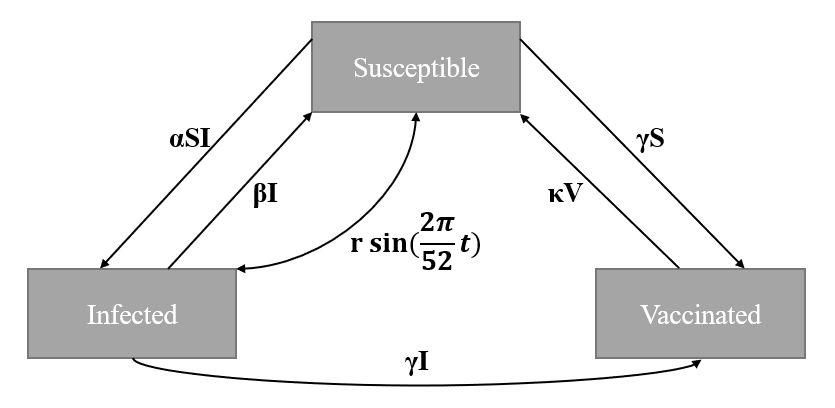
\includegraphics[width = \linewidth]{SIV_flowchart.PNG}
    \captionof{figure}{Flowchart of SIV compartmental model.}
\end{Figure}

\section{Solution of the Mathematical Problem}

Due to the presence of sine terms, we are unable to solve this system with the same methods as the SIS and SIR models -- the presence of time-dependent external forcing results in the system no longer having fixed points. For the purposes of solving the model (i.e., finding the fixed points), we will ignore the external forcing and solve for the behavior of the system without the sine terms. Thus we have the following system of equations, which we will denote as the ``non-forced SIV model":


\begin{equation}
\begin{aligned} \label{nonForce_siv}
\frac{dS}{dt} &= -\alpha S I + \beta I - \gamma S + \kappa V\\
\frac{dI}{dt} &= \alpha S I - \beta I - \gamma I\\
\frac{dV}{dt} &= \gamma S + \gamma I - \kappa V
\end{aligned}
\end{equation}

\subsection{Trivial Fixed point}

A trivial fixed point is to take the initial condition $(S, I, V) = (0, 0, 0)$, but that doesn't provide any useful mathematical or biological information. We can find other fixed points by analyzing the system with the Jacobian set to $0$. Note that, since we are ignoring the sine-terms, the trivial fixed point is always stable.

\subsection{``DFE" Fixed point}

Note that we can rewrite this system of equations as the following matrix:

$$
\begin{bmatrix}
\frac{dS}{dt} \\
\frac{dI}{dt} \\
\frac{dV}{dt}
\end{bmatrix} =
\begin{bmatrix}
(-\alpha I - \gamma) S + \beta I + \kappa V\\
\alpha SI + (-\beta - \gamma)I + 0 \\
\gamma S + \gamma I - \kappa V
\end{bmatrix}
$$

Thus, we can take the Jacobian of the non-forced SIV model as follows:
$$
J_f = \begin{bmatrix}
-\alpha I - \gamma & \beta & \kappa \\
\alpha I & -\beta - \gamma & 0 \\
\gamma & \gamma & -\kappa
\end{bmatrix}
$$

In mathematical epidemiology, we typically analyze a fixed point at disease-free equilibrium, or ``DFE" \citep{doi:10.1093/bmb/ldp038}. This fixed point occurs when the initial condition of the system is $(S, I, V) = (N_1, 0, N_2)$,  with $N = N_1 + N_2$, that is, the initial condition where there are no diseased individuals in the population, and thus the entire population is either susceptible or vaccinated. Note that, aside from the DFE fixed point, there is one globally stable fixed point known as ``endemic equilibrium" , in which there is equilibrium between all three compartments \citep{sun2010global}. Unlike the endemic fixed point, it is possible for the DFE fixed point to be unstable. If and when the DFE initial condition is unstable, then the system will globally tend towards endemic equilibrium.

Since the DFE initial condition suggests that the susceptible and vaccinated compartments are in equilibrium, we can find this fixed point by setting:
$$
\begin{aligned}
-\alpha S^* I^* + \beta I^* - \gamma S^* + \kappa V^* &= \gamma S^* + \gamma I^* - \kappa V^* \\
I^* &= 0 \\
 - 2 \gamma S^* &= - 2 \kappa V^* \\
 \hline \\
 S^* &= \frac{\kappa}{\gamma}V^* \\
 S^* + V^* &= N \\
 \frac{\kappa}{\gamma}V^* + V^* &= N \\
 (1 + \frac{\kappa}{\gamma})V^* &= N \\
 V^* &= \frac{N}{1 + \frac{\kappa}{\gamma}} \\
 \hline \\
 V^* &= \frac{\gamma}{\kappa}S^* \\
 V^* + S^* &= N \\
 \frac{\gamma}{\kappa}S^* + S^* &= N \\
 (1 + \frac{\gamma}{\kappa})S^* &= N \\
 S^* &= \frac{N}{1 + \frac{\gamma}{\kappa}}
\end{aligned}
$$
Thus, the DFE fixed point is given by $(S^*, I^*, V^*) = (\frac{N}{1 + \frac{\gamma}{\kappa}}, 0, \frac{N}{1 + \frac{\kappa}{\gamma}})$. As an example, Figure 2 demonstrates the long-run behavior of the non-forced SIV model given parameters $\alpha = 0.0035$, $\beta = 0.56$, $\gamma = 0.0056$, $\kappa = 0.0028$, and DFE initial conditions.

\begin{Figure}
    \centering
    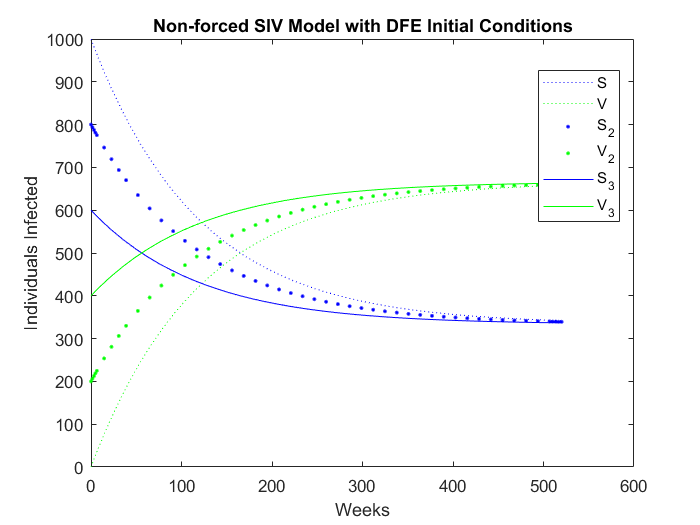
\includegraphics[width = \linewidth]{example_nonForced_siv_DFE.png}
    \captionof{figure}{Long-run behavior of non-forced SIV model with DFE initial conditions.}
\end{Figure}

Note that even when given different initial conditions, $S$ and $V$ tend to the fixed point at $(\frac{N}{1 + \frac{\gamma}{\kappa}}, 0, \frac{N}{1 + \frac{\kappa}{\gamma}})$, which should be approximately $(333, 0, 667)$ given our rate parameters.

Next, we will evaluate the stability of the DFE fixed point. Substituting in the DFE initial condition into the Jacobian gives us:

$$
J_f^{DFE}(N_1, 0, N_2) = \begin{bmatrix}
-\gamma & \beta & \kappa \\
0 & - \beta - \gamma & 0 \\
\gamma & \gamma & -\kappa
\end{bmatrix}
$$

We can find the eigenvalues of this matrix by taking the determinant and expanding upon the middle row:
$$
det(J_f^{DFE}(N_1, 0, N_2) - \lambda) = \begin{bmatrix}
-\gamma - \lambda & \beta & \kappa \\
0 & - \beta - \gamma - \lambda & 0 \\
\gamma & \gamma & -\kappa - \lambda
\end{bmatrix}
$$

This gives us
$$
\begin{aligned}
0 - (-\beta - \gamma - \lambda) \cdot det(\begin{bmatrix}
-\gamma - \lambda & \kappa \\
\gamma & -\kappa - \lambda
\end{bmatrix}) + 0 &= - (-\beta - \gamma - \lambda) \cdot det(\begin{bmatrix}
-\gamma - \lambda & \kappa \\
\gamma & -\kappa - \lambda
\end{bmatrix}) \\
&= (\beta + \gamma + \lambda)((-\gamma - \lambda) \cdot (-\kappa - \lambda)) - (\kappa \gamma) \\
&= (\beta + \gamma + \lambda)(\lambda ^2 + \kappa \lambda + \gamma \lambda + \kappa \gamma - \kappa \gamma) \\
&= (\beta + \gamma + \lambda)(\lambda^2 + \kappa \lambda + \gamma \lambda) \\
&= \lambda ^3 + (k + \gamma ^2 + 2\gamma + \beta) \lambda ^2 + (\beta \kappa + \beta \gamma + \kappa \gamma) \lambda
\end{aligned}
$$
Note that there is no constant term. Thus, we know that one of the eigenvalues is $0$. We can find the other two eigenvalues by factoring out a $\lambda \neq 0$. \\
$$
\begin{aligned}
\lambda ^3 + (k + \gamma ^2 + 2\gamma + \beta) \lambda ^2 + (\beta \kappa + \beta \gamma + \kappa \gamma) \lambda & \rightarrow \lambda ^2 + (k + \gamma ^2 + 2\gamma + \beta) \lambda + (\beta \kappa + \beta \gamma + \kappa \gamma) \\
\end{aligned}
$$

From here we use the quadratic formula to find the other two eigenvalues:
$$
\lambda ^2 + (\kappa + \gamma ^2 + 2\gamma + \beta) \lambda + (\beta \kappa + \beta \gamma + \kappa \gamma) = 0
$$
$$
\lambda = \frac{-(\kappa + \gamma ^2 + 2 \gamma + \beta) \pm \sqrt{(\kappa + \gamma^2 + 2\gamma + \beta)^2 - 4(\beta \kappa + \beta \gamma + \kappa \gamma)}}{2}
$$

Note that, as mentioned in \textit{Mathematical Model}, reasonable values of $\alpha$,  $\beta$, $\gamma$, and $\kappa$ are all much less than $1$. Thus, we can expect $(\kappa + \gamma ^2 + 2 \gamma + \beta)^2$ and $4(\beta \kappa + \beta \gamma + \kappa \gamma)$ to be fairly small numbers, such that $\sqrt{(\kappa + \gamma ^2 + 2 \gamma + \beta)^2 - 4(\beta \kappa + \beta \gamma + \kappa \gamma)} < \kappa + \gamma ^2 + 2 \gamma + \beta$. Also recall that all rate parameters are positive. Thus, the real component of the non-zero eigenvalues for the DFE initial condition is always negative, which suggests that, for the purposes of this model, this is always a stable fixed point.

\subsection{Endemic Fixed point}
Next, let us examine the endemic fixed point. We can solve for $S^*$ using the differential equation for $I$.
$$
\begin{aligned}
\alpha S^*I^* - \beta I^* - \gamma I^* &= 0 \\
\alpha S^*I^* &= \beta I^* + \gamma I^* \\
\alpha S^* &= \beta + \gamma \\
S^* &= \frac{\beta + \gamma}{\alpha}
\end{aligned}
$$
We can solve for $V^*$ using the differential equations for $S$ and $I$:
$$
\begin{aligned} 
-\alpha S^*I^* + \beta I^* - \gamma S^* + \kappa V^* &= 0\\
\alpha S^*I^* - \beta I^* - \gamma I^* &= 0 \\
\hline \\
-\alpha S^*I^* + \beta I^* - \gamma S^* + \kappa V^* + \alpha S^*I^* - \beta I^* - \gamma I^* &= 0 \\
\hline \\
- \gamma S^* + \kappa V^* - \gamma I^* &= 0\\
V^* &= \frac{\gamma(S^* + I^*)}{\kappa}
V^* &= \frac{\gamma(S^* + I^*)}{\kappa} \\
V^* &= \frac{\gamma}{\kappa}(N - V^*) \\
V^* &= \frac{\gamma}{\kappa}N - \frac{\gamma}{\kappa}V^* \\
(1 + \frac{\gamma}{\kappa})V^* &= N \\
V^* &= \frac{N}{1 + \frac{\gamma}{\kappa}}
\end{aligned}
$$

Now we can solve for $I^*$ using the definitions of $S^*$ and $V^*$ and the differential equation for $V$:
$$
\begin{aligned}
\gamma S^* + \gamma I^* - \kappa V^* &= 0 \\
\gamma I^* &= \kappa V^* - \gamma S^* \\
I^* &= \frac{\kappa }{\gamma}V^* - S^* \\
I^* &= \frac{\kappa}{\gamma}\frac{N}{1 + \frac{\gamma}{\kappa}} - \frac{\beta + \gamma}{\alpha}
\end{aligned}
$$

Thus, the endemic fixed point is given by $(S^*, I^*, V^*) = (\frac{\beta + \gamma}{\alpha}, \frac{\kappa}{\gamma}\frac{N}{1 + \frac{\gamma}{\kappa}} - \frac{\beta + \gamma}{\alpha}, \frac{N}{1 + \frac{\gamma}{\kappa}})$. 

Figure 3 demonstrates the long-run behavior of the non-forced SIV model given parameters $\alpha = 0.0035$, $\beta = 0.56$, $\gamma = 0.0056$, and $\kappa = 0.0028$ and non-DFE initial conditions.

\begin{Figure}
    \centering
    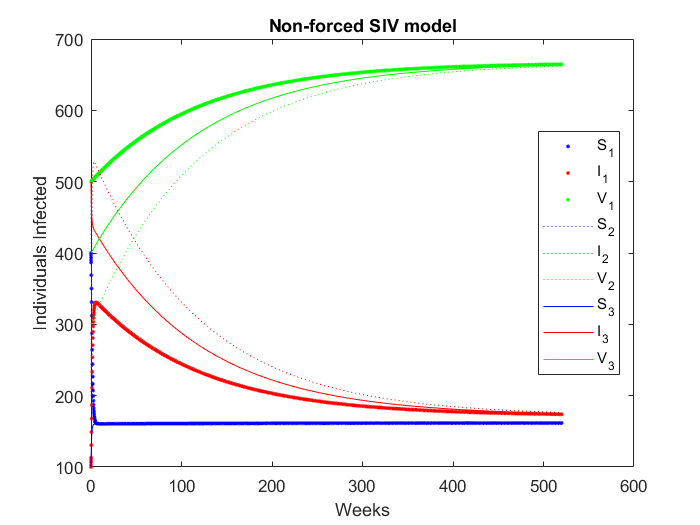
\includegraphics[width = \linewidth]{example_nonForced_siv_end.png}
    \captionof{figure}{Long-run behavior of non-forced SIV model.}
\end{Figure}

Note that regardless of initial conditions, $S$, $I$, and $V$ tend to the fixed point at $(\frac{\beta + \gamma}{\alpha}, \frac{\kappa}{\gamma}\frac{N}{1 + \frac{\gamma}{\kappa}} - \frac{\beta + \gamma}{\alpha}, \frac{N}{1 + \frac{\gamma}{\kappa}})$, which should be approximately $(161, 172, 667)$ given our rate parameters.

As previously mentioned, the endemic fixed point is globally stable, given reasonable rate parameters \citep{sun2010global}. The proof for why the endemic fixed point is globally stable involves a Lyapunov function and is beyond the scope of this course.

Although we cannot explicitly solve the system when including the external forcing, we can observe that the long-run behavior is still similar. Figure 4 demonstrates the long-run behavior of the forced SIV model given parameters $\alpha = 0.0035$, $\beta = 0.56$, $\gamma = 0.0056$, $\kappa = 0.0028$, and $r = 20$.

\begin{Figure}
    \centering
    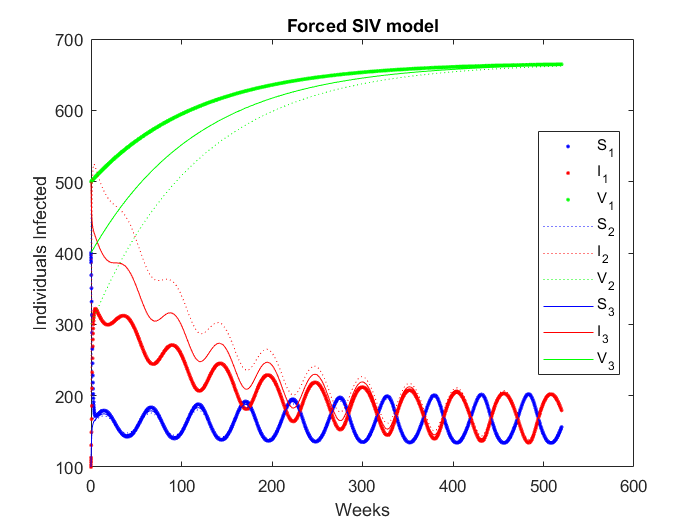
\includegraphics[width = \linewidth]{example_forced_siv_end.png}
    \captionof{figure}{Long-run behavior of forced SIV model.}
\end{Figure}

Note that it appears to reach periodic equilibrium around the same fixed points as in the non-forced SIV model. This may suggest that the long-run behavior of the forced SIV model cycles about the fixed points of the non-forced SIV model. Additionally, note that even when given different initial conditions, $S$, $I$, and $V$ still tend towards the same long-run behavior.



\section{Results and Discussion}

We will now discuss the application of this model in predicting the timing and intensity of seasonal Influenza. The Center for Disease Control reports that approximately 46.8\% of the population of the United States currently has an effective vaccine against seasonal Influenza \citep{flannery2017interim}. From this, we can estimate that approximately 53.2\% of the population is currently susceptible to Influenza. Additionally, the average number of people per week exhibiting symptoms of Influenza is roughly 178, drawn from data across the past 20 years \citep{centers2018weekly}. Furthermore, the maximum number of infected individuals recorded per week over the past 20 years is 3637 \citep{centers2018weekly}.

We will assume that there is a limit to the number of people that individuals can infect, due to geographical boundaries or otherwise. For the purposes of simulating infection dynamics in the United States, we will simulate a smaller sample population, with $N = 10000$. In order to have long-run behavior similar to the reported rates of vaccination and disease incidence, we will use the parameters $\alpha = 0.00001$, $\beta = 0.045$, $\gamma = 0.005$, $\kappa = 0.006$, and $r = 20$. Based off of our findings in \textit{Solution of the Mathematical Problem}, these parameters should result in long-run behavior with $S$, $I$, and $V$ approaching periodic equilibrium around $(\frac{\beta + \gamma}{\alpha}, \frac{\kappa}{\gamma}\frac{N}{1 + \frac{\gamma}{\kappa}} - \frac{\beta + \gamma}{\alpha}, \frac{N}{1 + \frac{\gamma}{\kappa}})$, which is approximately $(5000, 500, 4500)$.

Figure 5 details the SIV model using the informed parameters, as run with three different sets of initial conditions, being $(8000, 1000, 1000)$, ($1000, 2000, 7000$), and ($5500, 500, 4000$).

\begin{Figure}
    \centering
    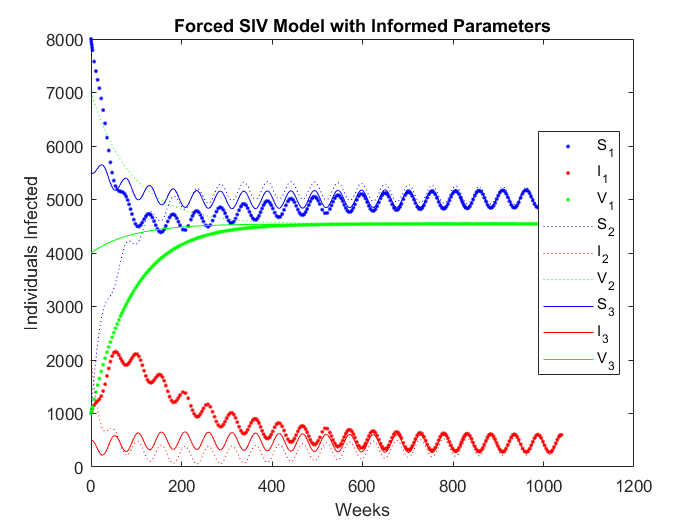
\includegraphics[width = \linewidth]{informed_siv.png}
    \captionof{figure}{SIV model with informed parameters over 20 years.}
\end{Figure}

Note that even when given different initial conditions, $S$, $I$, and $V$ tend towards periodic equilibrium around the fixed points of the non-forced SIV model. Additionally, in using informed parameters, the long-run behavior of the model somewhat resembles the published percentages of vaccination and disease incidence.

Figure 6 details clinical and epidemiological data published by the CDC regarding the number of individuals infected with seasonal Influenza, H3N2, each week from 1998 to 2018 \citep{centers2018weekly}.

\begin{Figure}
    \centering
    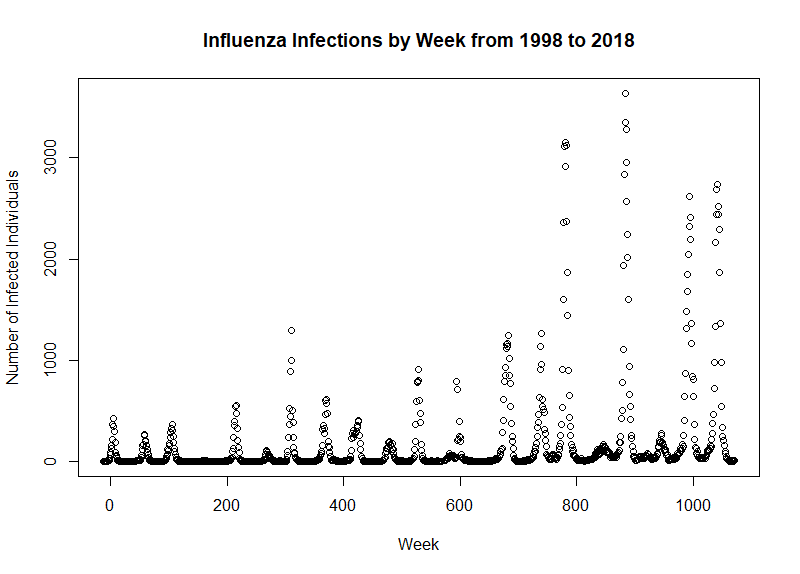
\includegraphics[width = \linewidth]{cdc_influenzaData.png}
    \captionof{figure}{Influenza infections by week from 1998 to 2018.}
\end{Figure}

The long-run behavior of the ``Infected" compartment in the SIV model somewhat resembles the clinical data published in literature. More specifically, the SIV model appears to be able to capture some elements of the seasonal behavior of Influenza, as seen in the periodicity of its long-run behavior. However, it appears that the SIV model was unable to capture relevant information about the varied intensity of seasonal outbreaks, as the amplitude of the external forcing is constant. This differs from the above clinical data, in which different years have seasonal outbreaks of varying intensity.

\section{Improvement}
It appears that a shortcoming of the SIV model is an inability to account for variation in the intensity of Influenza outbreaks -- the amplitude of external forcing is constant. This variance in intensity could possibly be explained by one of the biological or epidemiological implications that we ignored. For example, the SIV model is only capable of interpreting the behavior of one strain of Influenza. As mentioned in \textit{Simplifications}, a more realistic model would take into consideration multiple strains concurrently. When a certain strain has been dominant in Human populations for an extended period of time, individuals tend to more quickly lose immunity to the non-dominant strains \citep{bedford2015global}. A current example of this effect is seen between the H1N1 and H3N2 strains of Human Influenza -- H3N2 has been the dominant strain in Human populations for most recent years, but H1N1 has been shown to escape immune response at a faster rate \citep{lee2018deep}. One means of improving upon the SIV model would be take more of these biological and epidemiological assumptions into consideration, such that the model would be able to detect the factors that play into the varying intensity of Influenza outbreaks. This would likely make the model more accurate, however, it would also likely add additional parameters to the model, which would increase computational complexity. Adding parameters would also increase the number of decisions that must be made for the model.

Additionally, although the epidemiological behavior of seasonal influenza is periodic, the shape of the data shown in Figure 6 does not appear to resemble any sinusoidal curve. This suggests that a sine term is likely not the most appropriate function to represent the seasonal aspect of Influenza. The model could be improved by introducing a more suitable function to represent the external forcing associated with the seasonal behavior of influenza. A possible candidate for an alternative external forcing term could be a parabola.


\section{Conclusions}
We have presented a susceptible-infected-vaccinated model which attempts to take into consideration both the seasonal dynamics of Influenza as well as the time-limited immunity conferred through vaccination. Due to the presence of a time-dependent external forcing term, the fixed points of the system of ordinary differential equations could not be found, however, we were able to solve for the fixed points of the system when ignoring the periodic component. From this, we have shown that the long-run behavior of the ``forced SIV model" cycles about the fixed points of the ``non-forced SIV model". 

By consulting relevant literature as well as publicly available clinical and epidemiological data, we have identified a set of model parameters which result in output that somewhat resembles infection dynamics as observed in the past 20 years. Although the SIV model appears to have captured some elements of the seasonal behavior of Influenza infection dynamics, further work is necessary to account for the varying intensity of seasonal outbreaks.


\bigskip


\bibliographystyle{mbe}
\bibliography{references.bib}


\end{document}